\documentclass{assignment}
\usepackage{amsmath}
\usepackage{lipsum}
\usepackage{multicol}
\usepackage{fancyhdr}
\usepackage{graphicx}
\usepackage{blindtext}
\usepackage[dvipsnames]{xcolor}
\usepackage{enumitem}
\usepackage{cleveref}
\usepackage{color,soul}
\usepackage{amsfonts}
\usepackage{tikz}
\usepackage{algorithm}
\usepackage{algpseudocode}
\usetikzlibrary{positioning}

\newcommand{\indicator}[1]{\mathbf{1}_{\{#1\}}}
\usepackage{xparse}

% Define a new command for PDFs with subscripts
\NewDocumentCommand{\pdf}{ m }{f_{#1}(#1)}
\NewDocumentCommand{\indp}{}{\perp\!\!\!\!\perp}

\def\code#1{\texttt{#1}}
\newtheorem{anm}{Anm}

\begin{document}


\assignmentTitle
{Lucas Frykman}{0210127650}
{SF1930}
{Liam Solus}
{assets/KTH_logga.png}
{Statistisk inlärning och dataanalys}
{Projekt}

% \section*{Introduktion}
% Vi betraktar den skateboard tävlingen.

\section{Uppvärmning}



\begin{figure}[!h]
    \caption{Histogram av betyg skalad mellan 0 och 1}
    \begin{center}
        \includegraphics[width = 99mm]{assets/Figure_2.png} \label{Histogram 1}
    \end{center}
\end{figure}


Låt $B$ vara betyg för en ett skateboardåkare och trick. Vi vill skatta $P(B>0.6|B>0) = \frac{P(B>0|B>0.6)P(B>0.6)}{P(B>0)}=\frac{P(B>0.6)}{P(B>0)}$
som $\tilde{P}(B>0.6|B>0) = \frac{\sum_{i}^4\sum_{j}^{96}trick_{ij}\indicator{[0.6,1]}}{\sum_{i}^4\sum_{j}^{96}trick_{ij}\indicator{[0,1]}} \approx 0.96$
Det här stämmer med utseendet på \cref{Histogram 1}. När man plottar run 2 mot run 1 ser de ut att ha jätte svag korrelation \cref{Spridningsdiagram}

\begin{figure}
    \caption{Spridningsdiagram mellan run 1 och run 2}
    \begin{center}
        \includegraphics[width = 99mm]{assets/Figure_1.png}
    \end{center}
    \label{Spridningsdiagram}
\end{figure}


\section{En frekventistisk modell}
\begin{anm} \label{properties}
    Vår model för $X_i$ är följande 
    \\ $X_i = \left\{\begin{matrix}
        0 \text{ om } V_i=0
        \\ Z_i \text{ om } V_i=1
    \end{matrix}\right.$
    \\ där $V_i \sim \text{Ber}(\theta_i)$ och $Z_i\sim \text{Beta}(\alpha_i,\beta_i)$ det här är ekvivalent med att säga
    \\ $V_i = \indicator{x\neq0}(X_i)$ och $Z_i= X_i|(V_i=1)$ 
    \\ eftersom det här är bara en transformation av stokatiska variebler ger stickprov från $X_i$ oss ett stickprov för $Z_i$ och $V_i$
\end{anm}

\subsection*{(a) Skatta $\theta_{i}$}

Låt $x_{i[n]} = (x_{i1},x_{i2},...x_{in})^T$ vara vår stickprov från samtliga trick skateboardåkaren $i$ utförde.
\begin{align}
    L(\theta_{i},\alpha_{i},\beta_{i}|x_{i[n]}) = \prod_{j=1}^nf_{x_{i}}(x_{ij}) = \prod_{j}^n (1-\theta_i) \indicator{x=0} (x_{ij}) + \theta_if_{Z_i}(x_{ij})\indicator{x\neq0}(x_{ij})
    \\ \Longleftrightarrow \nonumber
    \\ L(\theta_{i},\alpha_{i},\beta_{i}|x_{i[n]}) = (1-\theta_i)^{n-m}\theta_i^{m}\prod_{j=1}^n\left(f_{Z_i}(x_{ij})\indicator{x\neq0}(x_{ij}) + \indicator{x=0}(x_{ij})\right) 
\end{align}
där $m=\sum_{j=1}^n \indicator{x\neq0}(x_{ij})$ alltså hur många gånger $x_{i}$ inte är noll (gånger tävlaren $i$ landade tricket).
Nu tar vi log likliehoodfunktionen.
\begin{align}
    \Longrightarrow \log(L) = (n-m)\log(1-\theta_i)+m\log(\theta_i)+ \sum_{j=1}^n \log \left(f_{Z_i}(x_{ij})\indicator{x\neq0}(x_{ij}) + \indicator{x=0}(x_{ij})\right) \label{loglike}
    \\ \Longleftrightarrow \partial_{\theta_i}\log(L) = \frac{m-n}{1-\theta_i} + \frac{m}{\theta_i} = 0 \label{blah}
    \\ \Longleftrightarrow \frac{m-n\theta_i}{\theta_i(1-\theta_i)} = 0 \Longleftrightarrow \hat{\theta_i} = \frac{m}{n} \label{MLE result}
\end{align}
MLE för bernoulli fördelningens $V_i$ parameter $\hat{\theta_i} = \text{argmax}_{\theta\in\Omega} L(\theta_i|v_{i[n]}) = \bar{v_i}$ skulle ge oss samma resultat. Eftersom vi kan transformera stickprovet $x_{i[n]}\rightarrow v_{i[n]}$ med \cref{properties} $v_i=\indicator{x\neq0}(x_i)$.
vilket betyder att $m=\sum_{j=1}^n v_i$ och därmed får \cref{MLE result} att sammanfalla med MLE av bernoulli fördelningen. 
\subsection*{(b) skatta $\alpha_i$ och $\beta_i$}
Observera att från \cref{loglike}  $\sum_{j=1}^n \log \left(f_{Z_i}(x_{ij})\indicator{x\neq0}(x_{ij}) + \indicator{x=0}(x_{ij})\right) = \sum_{j=1}^n \log \left(f_{Z_i}(x_{ij})\indicator{x\neq0}(x_{ij})\right)$ eftersom $\log(1)=0$.
Vi vet att 
\\ $\text{argmax}_{\alpha,\beta\in\Omega}\log(L)=\text{argmax}_{\alpha,\beta\in\Omega}\sum_{j=1}^n \log \left(f_{Z_i}(x_{ij})\indicator{x\neq0}(x_{ij})\right)$ vilket är ekvivalent med 
\\$\text{argmax}_{\alpha,\beta\in\Omega} \log(L(\alpha,\beta|z_{i[k]}))$ för att $z$ stickprovet innehåller alla trick som landade $z_{i[k]}=(z_{i1},\dots z_{ik})^T = \left\{x_{ij}\in x_{i[n]} : x_{ij}\neq 0\right\}$
\\ Vi ska alltså bara maximera log-likelihood av beta fördelningens paramtrerna givet data from $Z_i$

\begin{align*}
    \left\{\begin{matrix}
        \partial_{\alpha}\log(L(\alpha,\beta|z_{i[k]})) = \sum_{j=1}^k \partial_\alpha \log(f(z_{ij})) = 0
        \\ \\ \partial_{\beta}\log(L(\alpha,\beta|z_{i[k]})) = \sum_{j=1}^k \partial_\beta \log(f(z_{ij})) = 0
        \end{matrix}\right.
    \\ 
    \\ \text{:: } \partial_\alpha\log(f(z_{ij})) = \partial_\alpha\log \left( \frac{\Gamma(\alpha + \beta)}{\Gamma(\alpha) \cdot \Gamma(\beta)} \cdot z_{ij}^{\alpha-1} \cdot (1-z_{ij})^{\beta-1}\right) 
    \\  = \partial_\alpha \left(\log \Gamma(\alpha + \beta) - \log\Gamma(\alpha) - \log \Gamma(\beta) + (\alpha-1) \log z_{ij} + (\beta-1)\log (1-z_{ij}) \right)
    \\  = \partial_\alpha\log(f(z_{ij})) = \psi(\alpha+\beta) - \psi(\alpha) + \log z_{ij} \text{  där  } \psi = \Gamma ' / \Gamma 
    \\ \left(\text{Vi gör liknande för } \partial_\beta \log f(z_{ij}) \right)
    \\ \Rightarrow 
    \left\{\begin{matrix}
        \partial_{\alpha}\log L= k\psi(\alpha+\beta)-k\psi(\alpha) + \sum_{j=1}^k\log(z_{ij}) = 0
        \\ \\ \partial_{\beta}\log L= k\psi(\alpha+\beta)-k\psi(\beta) + \sum_{j=1}^k\log(1-z_{ij})) = 0
        \end{matrix}\right.
\end{align*}
\\ Det går dock inte att lösa ML skattningen analytisk härifrån. Numeriska metoder som newton rhapson eller gradient descent
behövs för att skatta vår ML skattning. Att göra så medför sig en del problem som ökar systematiska felet genom
numerisk fel. Vi behåller riktighet i punktskattningen genom att använda moment metoden istället. Vi utgår från följande
system ekvationerna
\begin{align*}
    \left\{\begin{matrix}
        M_1(\mathbf{Z}_i)  = \text{E}[Z_i]
        \\ M_2(\mathbf{Z}_i) = \text{Var}[Z_i]+\text{E}[Z_i]^2
    \end{matrix}\right.
    \Longleftrightarrow \left\{\begin{matrix}
        \Leftrightarrow M_1 = \frac{\alpha}{\alpha+\beta}
        \\ M_2 = \frac{\alpha\beta}{(\alpha+\beta)^2(\alpha+\beta+1)}+(\frac{\alpha}{\alpha+\beta})^2
    \end{matrix}\right.
    \\ :: S^2=\frac{1}{n}\sum (Z_{k}-\bar{Z})^2 = M_2-M_1^2
    \\ \Longleftrightarrow \left\{\begin{matrix}
        \Leftrightarrow \alpha = \beta\frac{M_1}{1-M_1}
        \\ S^2 = \frac{\alpha\beta}{(\alpha+\beta)^2(\alpha+\beta+1)}
    \end{matrix}\right.
    \Longleftrightarrow \left\{\begin{matrix}
        \widetilde{\alpha} = M_1\left(\frac{M_1(1-M_1)}{S^2}-1\right)
        \\ \widetilde{\beta} = (1-M_1)\left(\frac{M_1(1-M_1)}{S^2}-1\right)
    \end{matrix}\right.
    \\ = \left\{\begin{matrix}
        \widetilde{\alpha_i} = \bar{Z_i}\left(\frac{\bar{Z_i}(1-\bar{Z_i})}{S^2}-1\right)
        \\ \widetilde{\beta_i} = (1-\bar{Z_i})\left(\frac{\bar{Z_i}(1-\bar{Z_i})}{S^2}-1\right)
    \end{matrix}\right.
\end{align*}
För vissa skatebordåkare kan man inte få en punktskattningen eftersom det finns endast en
datapunkt $z_1$ för vissa skatebordåkare. Stickprovsvariansen i sådana fall blir lika med noll. Stickprovsvariansen
representerar hur osäkert vi är om en skatebordåkares prestation på en trick. Intuivt sett Vi gör valet
här att skatta stickprovsvariansen som $S_i^2\approx \bar{S^2}$ dvs vi tar medelvärdet av samtliga varianser. 
\subsection*{(c) Model för $Y_i$}
$Y_i$ ska vara run betyget för åkaren $i$. Eftersom $Y_i\in(0,1]$ (varje deltagare får betyg större än 0) 
kommer bernoulli delen försvinna. Men annars fungerar en run ganska liknande som en trick. 
Så vi antar att $Y_i\sim \text{Beta}(^y\alpha_i,^y\beta_i)$. 
För att skatta parameter till $Y$ använder vi samma moment metoden som vi använde för att skatta $\alpha,\beta$ för $X$.
(Obs: Enda skillnaden i det här fallet vi slipper använda medelvärdet på stickprovsvariansen $S^2=\bar{S^2}$
för att det är garanterat vi får mer än en datapunkt för alla skateboardåkare $i$.)
\subsection*{(d) Simulering}
Total betyget för varje deltagare beräknas som summan av deras två största trick betyg och största run betyg. Vi
kan beskriva i termer av stokatiska variabler. Låt $O_i$ vara total betyg för deltagare $i$.
Låt $Q_{i,\text{först}}=\max(X_{i1},X_{i2},X_{i3},X_{i4})$ och 
\\$Q_{i,\text{andra}}=\max(\min(X_{i1}, X_{i2}), \min(X_{i1}, X_{i3}), \min(X_{i1}, X_{i4}), \min(X_{i2}, X_{i3}), \min(X_{i2}, X_{i4}), \min(X_{i3}, X_{i4}))$.
\\Vi vill simulera total betyget för varje deltagare $i$ som $O_i=Q_{i,\text{först}}+Q_{i,\text{andra}}+\max(Y_{i1},Y_{i2})$
De som fick de 4 högsta betyg får delta i finalen. Vi simulerar $5000$ LCQ:ar. Det ger oss en följd av stokatisk sets $\mathbf{W}_1,...\mathbf{W}_{5000}$.
Python har redan libraries för att generera stickprov från beta och bernoulli fördelningar. Så vi slipper 
använda box muller, inverse metoden, eller dylikt. 
\begin{figure}
    \caption{Frequency appearing in final $\mathbf{W}$}
    \begin{center}
        \includegraphics[width = 200mm]{assets/freq_bar_graph.png} 
    \end{center}
    \label{Histogram 2}
\end{figure}
Jag skapade en frequency bar graph för att visualisera simuleringen och fick detta i en körning \cref{Histogram 2}.
De som har markerats i orange är de som faktiskt vann den verkliga LCQ:en.
Typvärdet på $\mathbf{W}$ innehöll oftast Hoban, Eaton, Jordan, och Shirai. Typvärdets frekvens vara kring 50 gger dvs $1\%$. 
Frekvensen av när $\mathbf{W}$ innehöll samtliga verkliga vinnare (nämligen Gustavo, Hoban, Eaton, Decenzo) vara när 16-20 gger dvs mindre än $0.5\%$.  

\newpage 
\section{En bayesiansk modell}
\subsection*{(a) Apriori fördelnignar}
Vi ska föreslå en simultan apriori fördelningn för $[\Theta_i,A_i,B_i]^T$.
\\ \textbf{Apriori för $\Theta$}
\\ Vi vet att $\theta$ representerar hur pass sannolikt det är att skatebordåkaren landar tricket och att det är ett värde mellan 0 och 1. 
Vi har dock inga starka åsikter om $\theta$ innan vi observerar datan. Därför använder vi en
icke-informativ apriori.
\\ $\pdf{\theta_i}\propto 1$
\\ \textbf{Apriori för $A,B$}
\\ Vi har inte någon vettig anledning att anta $A\indp B$ så vi behöver en egentlig simultan fördelning
som har stöd $\alpha,\beta \in (0,\infty]\times (0,\infty]$.
För att uppnå detta omformulerar vi fördelningen med avseende på dess medelvärde $\mu$ och en mått på precision $\kappa$. Det vill säga, för $X\sim\mathrm{Beta}(\alpha, \beta)$ tar vi
$$\mu = \frac{\alpha}{\alpha + \beta} \text{ och } \kappa = \alpha + \beta + 1$$

$\kappa$ är ett mått på precision för fördelningen eftersom det är omvänt proportionellt mot variansen:
$$
\mathrm{Var}[X] = \frac{\alpha\beta}{(\alpha + \beta)^2(\alpha + \beta + 1)} = \frac{\mu(1 - \mu)}{\kappa}.
$$
Vi kan sedan ange en fördelning $[\mu, \kappa]^T$ (enligt en hierarki) och sedan omvandla denna
fördelning tillbaka till parametrarna $\alpha$ och $\beta$ för att få en fördelning för $[A, B]^T$.
Vi tar den hierarkiska modellen:
$$\kappa | \mu \sim \mathrm{Gamma}(\theta, \lambda),\mu \sim \mathrm{U}(0,1)$$
En variabelbyte ger oss den priorfördelning för parametrarna $\alpha$ och $\beta$:
$$f_{A, B}(\alpha, \beta) = \frac{\lambda^\theta}{\Gamma(\theta)}(\alpha + \beta + 1)^{\theta - 1}e^{-\lambda(\alpha + \beta + 1)}(\alpha + \beta)^{-1}.$$
%\\$\pdf{\alpha_i,\beta_i} = \frac{\lambda^\theta}{\Gamma(\theta)}(\alpha_i+\beta_i+1)^{\theta-1}e^{-\lambda(\alpha_i+\beta_i+1)}(\alpha_i+\beta_i)^{-1}$  
\\Vi antar $\Theta_i \indp A_i,B_i$ för alla $i$ $\Longrightarrow \pdf{\theta_i,\alpha_i,\beta_i} = \pdf{\theta_i}\pdf{\alpha_i,\beta_i}$ 
\subsection*{(b) Aposteriori för $X_i$ och skattning} 
$\pdf{\theta_i, \alpha_i,\beta_i|x_i} \propto \pdf{\theta_i}\pdf{\alpha_i,\beta_i} \pdf{x_i|\theta_i,\alpha_i,\beta_i}$
\\ Vårt mål är att använda aposteriorin för att skatta $\text{E}[\Theta_i,A_i,B_i|\mathbf{X_i}=\mathbf{x_i}]$.
För att göra detta använder vi metropolis algoritimen för att generera ett stickprov och ta stickprovsmedelvärdet
$$\begin{pmatrix} \theta_{i0},\theta_{i1} \dots \theta_{i5000}\\ \alpha_{i0},\alpha_{i1}\dots \alpha_{i5000}  \\ \beta_{i0},\beta_{i1}\dots \beta_{i5000}\end{pmatrix} \longrightarrow
\begin{pmatrix}
    \bar{\theta_i} \\
    \bar{\alpha_i} \\
    \bar{\beta_i}
\end{pmatrix}$$  
Aposteriorin är vår målfördelning men vi kommer använda $L_{p}(\theta_i, \alpha_i,\beta_i) \propto \log(\pdf{\theta_i, \alpha_i,\beta_i|\mathbf{x}_i})$ istället.
Data fördelning $\pdf{\mathbf{x}_i|\theta_i, \alpha_i,\beta_i}$ i aposterorin är samma som likelihoodfunktionen 
$L(\theta_i, \alpha_i,\beta_i|\mathbf{x}_i)$
$$
\Rightarrow L_p(\theta_i, \alpha_i,\beta_i) = \underbrace{\log(\pdf{\theta_i)}}_{\log(1)=0}+\log(\pdf{\alpha_i,\beta_i})+\log L(\theta_i,\alpha_i,\beta_i)
$$
 
\begin{algorithm}
    \caption{Metropolis Algorithm}
    \begin{algorithmic}[1]
    \State Initialize the chain with  $\mathbf{\Theta}_0=[\theta_{i0},\beta_{i0},\alpha_{i0}]^T$
    \For{$k = 1$ to $5000$} \Comment{Iterate for a total of $5000$ steps}
    \State Generate a proposal state $\mathbf{\Theta}'$ from a proposal distribution $Q(\mathbf{\Theta}' | \mathbf{\Theta}_{k-1})$
    \State Calculate the acceptance ratio $R = \min\left(1, \frac{L_p(\mathbf{\Theta}')}{L_p(\mathbf{\Theta}_{k-1})}\right)$, where $L_p(\mathbf{\Theta})$ is the target distribution
    \State Generate a uniform random number $u \sim \text{Uniform}(0, 1)$
    \If{$u \leq R$}
    \State Accept the proposal: $\mathbf{\Theta}_k = \mathbf{\Theta}' $
    \Else
    \State Reject the proposal: $\mathbf{\Theta}_{k}  = \mathbf{\Theta}_{k-1}$
    \EndIf
    \EndFor
    \end{algorithmic}
\end{algorithm}
Valet för förslagsfördelning blir $\Theta'\sim Q(\theta'|\theta_{k-1}) = 
\begin{pmatrix}
    \exp(\log \alpha_{k-1} + \delta Z_\alpha)
    \\ \exp(\log \beta_{k-1} + \delta Z_\beta)
    \\ U_\theta
\end{pmatrix}$
där $Z_\alpha \sim \text{N}(0,1)$, $Z_\beta \sim \text{N}(0,1)$, $U_\theta \sim \text{U}(0,1)$, och $\delta = 0.5$

\newpage
\subsection*{(c) Aposteriori för $Y_i$}
Eftersom $Y_i \sim \text{Beta}(^y\alpha_i,^y\beta_i)$ ska vi använda en apriori fördelning av samma form som den alpha beta apriori i $X$.
\\ $\pdf{\alpha_i,\beta_i} = \frac{\lambda^\theta}{\Gamma(\theta)}(\alpha_i+\beta_i+1)^{\theta-1}e^{-\lambda(\alpha_i+\beta_i+1)}(\alpha_i+\beta_i)^{-1}$  
som ger oss aposteriorin 
$$\pdf{\alpha_i,\beta_i|\mathbf{y}_i}\propto \pdf{\alpha_i,\beta_i}\pdf{\mathbf{y}_i|\alpha_i,\beta_i}$$
\subsection*{(d) Simulering för bayesiansk modell}
Jag använde $\begin{pmatrix} \bar{\theta_i} \\ \bar{\alpha_i} \\ \bar{\beta_i} \end{pmatrix}$ från metropolis som min punktskattning.  
\subsection*{(e) Teori}
\begin{figure}
    \centering
    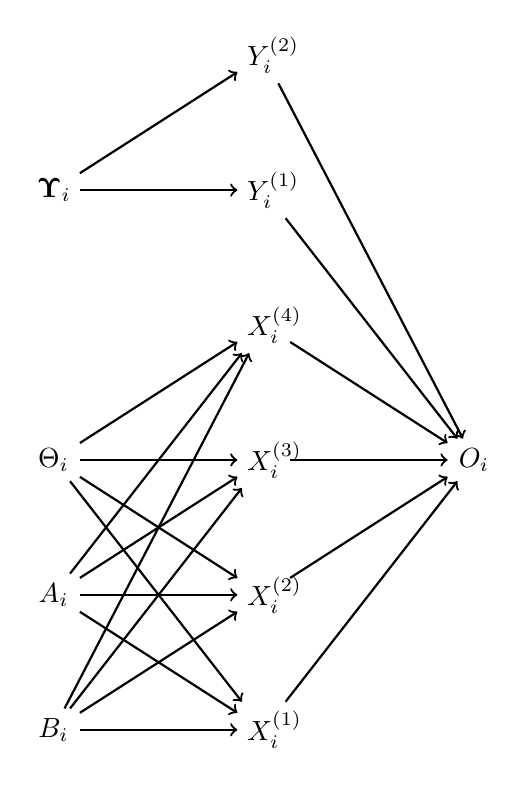
\begin{tikzpicture}[
        node/.style={minimum size=12pt, text width=12pt, align=center},
        edge/.style={->, thick, black},
    ]    
    \node[node] (1) at (0, 0) {$X_i^{(1)}$};
    \node[node, above=1cm of 1] (2) {$X_i^{(2)}$};
    \node[node, above=1cm of 2] (3) {$X_i^{(3)}$};
    \node[node, above=1cm of 3] (4) {$X_i^{(4)}$};
    \node[node, above=1cm of 4] (5) {$Y_i^{(1)}$};
    \node[node, above=1cm of 5] (6) {$Y_i^{(2)}$};
    \node[node, left=2cm of 5] (7) {$\mathbf{\Upsilon}_i$};
    \node[node, left=2cm of 3] (8) {$\Theta_i$};
    \node[node, left=2cm of 2] (9) {$A_i$};
    \node[node, left=2cm of 1] (10) {$B_i$};
    \node[node, right=2cm of 3] (11) {$O_i$};
    
    \draw[edge] (7) -- (5);
    \draw[edge] (7) -- (6);
    \draw[edge] (8) -- (1);
    \draw[edge] (8) -- (2);
    \draw[edge] (8) -- (3);
    \draw[edge] (8) -- (4);
    \draw[edge] (9) -- (1);
    \draw[edge] (9) -- (2);
    \draw[edge] (9) -- (3);
    \draw[edge] (9) -- (4);
    \draw[edge] (10) -- (1);
    \draw[edge] (10) -- (2);
    \draw[edge] (10) -- (3);
    \draw[edge] (10) -- (4);
    \draw[edge] (1) -- (11);
    \draw[edge] (2) -- (11);
    \draw[edge] (3) -- (11);
    \draw[edge] (4) -- (11);
    \draw[edge] (5) -- (11);
    \draw[edge] (6) -- (11);
    \end{tikzpicture}
    \caption[short]{acyklisk riktad graf}
\end{figure}

\newpage
\section{En bayesiansk modell med en hierarki}
\subsection*{(a) Apriori fördelning för $\theta$} 
\subsection*{(b) Aposteriori för $X_i$}
\subsection*{(c) Aposteriori för $Y_i$}
\subsection*{(d) Simulering}
\subsection*{(e) Grafisk model}
\section{Diskussion}

% \section{Kod}
% \lstinputlisting[language=Matlab,caption=foo]{assets/tmp.m} 
\end{document}
